%
% `template_basic.tex' - A bare-bones example of using the AIAA class.
%                        For a more advanced usage, see `template_advanced.tex'.
%
% Typical processing for PostScript (PS) output:
%
%  latex template_basic
%  latex template_basic   (repeat as needed to resolve references)
%
%  xdvi template_basic    (onscreen draft display)
%  dvips template_basic   (postscript)
%  gv template_basic.ps   (onscreen display)
%  lpr template_basic.ps  (hardcopy)
%
% With the above, only Encapsulated PostScript (EPS) images can be used.
%
% Typical processing for Portable Document Format (PDF) output:
%
%  pdflatex template_basic
%  pdflatex template_basic      (repeat as needed to resolve references)
%
%  acroread template_basic.pdf  (onscreen display)
%
% If you have EPS figures, you will need to use the epstopdf script
% to convert them to PDF because PDF is a limmited subset of EPS.
% pdflatex accepts a variety of other image formats such as JPG, TIF,
% PNG, and so forth -- check the documentation for your version.
%
% If you do *not* specify suffixes when using the graphicx package's
% \includegraphics command, latex and pdflatex will automatically select
% the appropriate figure format from those available.  This allows you
% to produce PS and PDF output from the same LaTeX source file.
%
% To generate a large format (e.g., 11"x17") PostScript copy for editing
% purposes, use
%
%  dvips -x 1467 -O -0.65in,0.85in -t tabloid template_basic
%
% For further details and support, read the Users Manual, aiaa.pdf.
%
% This software is released under the terms of the LaTeX Project Public
% License.  Copyright (C) 2004 by Bil Kleb, Bill Wood, and Erich Knausenberger.

\documentclass[]{aiaa-tc}% insert '[draft]' option to show overfull boxes

 \title{Bare-Bones \LaTeX\ Template for\\
        AIAA Technical Conference Papers}

 \author{
  First A. Author%
    \thanks{Job Title, Department, Address, and AIAA Member Grade.}
  \ and Second B. Author\thanksibid{1}\\
  {\normalsize\itshape
   Business or Academic Affiliation, City, Province, Zipcode, Country}\\
  \and
  Third C. Author%
   \thanks{Job Title, Department, Address, and AIAA Member Grade.}\\
  {\normalsize\itshape
  Business or Academic Affiliation, City, Province, Zipcode, Country}
 }

 % Data used by 'handcarry' option if invoked
 \AIAApapernumber{YEAR-NUMBER}
 \AIAAconference{Conference Name, Date, and Location}
 \AIAAcopyright{\AIAAcopyrightD{YEAR}}

 % Define commands to assure consistent treatment throughout document
 \newcommand{\eqnref}[1]{(\ref{#1})}
 \newcommand{\class}[1]{\texttt{#1}}
 \newcommand{\package}[1]{\texttt{#1}}
 \newcommand{\file}[1]{\texttt{#1}}
 \newcommand{\BibTeX}{\textsc{Bib}\TeX}

\begin{document}

\maketitle

\begin{abstract}
This section introduces an approach that facilitates onboard mission planning and
task execution by an autonomous UAV. The ultimate goal of this design is to enable
near real-time mission planning or its rapid modification should the operational
conditions change and need arise. As soon as the mission objectives are defined by
the high level cognitive components, then the set of specific tasks targeting an
application of the UAV in a priory given operational environment, needs to be
designed. The task should specify the trajectory (both the path and the velocity
profile) such that the mission objectives are achieved, the UAV and its payload do
not exceed the flight dynamics constraints, and that the operational constraints such
as radar detection, airspace deconfliction and collision avoidance conditions are
met. Thus, this section outlines a path generation approach that is suitable for near
real-time computation of feasible trajectories for a single UAV that accounts for the
flight dynamics and operational constraints, and can be followed by resorting to the
path following algorithm\cite{JGCD10_PFL1aug}.
\end{abstract}

\section*{Nomenclature}

\begin{tabbing}
  XXX \= \kill% this line sets tab stop
  $J$ \> Jacobian Matrix \\
  $f$ \> Residual value vector \\
  $x$ \> Variable value vector \\
  $F$ \> Force, N \\
  $m$ \> Mass, kg \\
  $\Delta x$ \> Variable displacement vector \\
  $\alpha$ \> Acceleration, m/s\textsuperscript{2} \\[5pt]
  \textit{Subscript}\\
  $i$ \> Variable number \\
 \end{tabbing}


\section{Feasible Path Generation}
This section introduces an approach that facilitates onboard mission planning and task
execution by an autonomous UAV. The ultimate goal of this design is to enable near
real-time mission planning or its rapid modification should the operational conditions
change and need arise. As soon as the mission objectives are defined by the high level
cognitive components, then the set of specific tasks targeting an application of the
UAV in a priory given operational environment, needs to be designed. The task should
specify the trajectory (both the path and the velocity profile) such that the mission
objectives are achieved, the UAV and its payload do not exceed the flight dynamics
constraints, and that the operational constraints such as radar detection, airspace
deconfliction and collision avoidance conditions are met. Thus, this section primarily outlines a
path generation approach that is suitable for near real-time computation of feasible
trajectories for a single UAV that accounts for the flight dynamics and operational
constraints, and can be followed by resorting to the path following
algorithm\cite{JGCD10_PFL1aug}.

Consider a single UAV that is tasked to fly a typical mission while avoiding detection
by an a priory known set of radars; the UAV performs its mission starting from its
current state (initial conditions) and arriving to the final conditions specified by
the mission planner. While the exact duration of the mission is not know a priory, it
is quite typical that the duration needs to be minimized; this can be justified by the
nature of the mission itself and/or the restrictions on energy expenditures imposed by
the UAV platform. Furthermore, suppose the objective of the UAV task is not only to
minimize the mission duration or the vehicle energy expenditures while meeting
dynamical constraints (e.g. bounds on maximum accelerations), but also to minimize the
probability of being detected by a number of radars.

The described problem belongs to the class of optimal control problems and it would be
desirable to have an algorithm capable of solving it in near real time. Unfortunately,
classical indirect approaches of calculus of variations (Bellman’s dynamic programming,
Pontrjagin’s maximum principle) can handle only very simple problems like a double
integrator where even an analytical solution is possible. However, obtaining an optimal
solution off-line for more realistic system is still quite difficult. That is why
various simplifying approaches have been developed to provide a near-optimal solution
in close to real-time rather than optimal solution (collocation method, method of
differential inclusions, etc.) off-line.

This work adopts the key idea of the approach proposed in Ref.\cite{JGCD00_Yakimenko}.
The method is based on explicit separation of the path and the velocity associated with
it. Both, the path and the velocity profile are represented by using some reference
functions expressed via a limited number of variable parameters such as, for example,
length of the path. The remaining states and controls can be determined using inverse
dynamics of original non-linear equations driving the system. As soon as the values of
variable parameters are fixed, then the path and the associated velocity profile are
given, and the required controls can be quickly evaluated using the inverse dynamics.
When done, a cost function representing the objective of the optimization task can be
calculated. Implementing this procedure iteratively enables calculating the best
solution (path and velocity profile) by varying a limited number of variable
parameters. The following brief explanation outlines the key elements of this approach
related to the tactical components of the cognitive mission planner. For detailed
presentation of the approach and its historical evolution an interested reader is
referred to the publication\cite{JGCD00_Yakimenko}and the references herein.

Thus, the approach to path generation exploits decoupling of spatial and temporal
specifications. Let $p_c(\tau) = [x(\tau), y(\tau), z(\tau)]^{\top}$ denote a desired
path to be followed by a single UAV in 3D space, parameterized by $\tau \in [0,
\tau_f]$. For computational efficiency, assume each coordinate $x (\tau), y(\tau),
z(\tau)$ is represented by an algebraic polynomial of degree $N$ of the form
\begin{eqnarray} \label{algpolynomials}
x_{i}(\tau) &=& \sum_{k = 0}^{N} a_{ik} \tau^k, \qquad i = 1,2,3,
\end{eqnarray}
where we set $x_{1} = x, x_{2} = y, x_{3} = z$ for notational convenience. The degree
$N$ of polynomials $x_{i}(\tau)$ is determined by the number of boundary conditions
that must be satisfied. Notice that these conditions (that involve spatial derivatives)
are computed with respect to the parameter $\tau$; this parameter will be later related
to actual temporal derivatives. Let $d_0$ and $d_f$ be the highest-order of the spatial
derivatives of $x_{i}(\tau)$ that must meet specified boundary constraints at the
initial and final points of the path, respectively. Then, the minimum degree $N^*$ of
each polynomial in (\ref{algpolynomials}) is $N^{*} = d_0 + d_f + 1$. For example, if
the desired path includes constraints on initial and final positions, velocities, and
accelerations (second-order derivatives), then the degree of each polynomial is $N^{*}
= 2 + 2 + 1 = 5$. Explicit formulae for computing boundary conditions $p'_c(0),
p''_c(0)$ and $p'_c(\tau_f), p''_c(\tau_f)$ are given later in this section. Additional
degrees of freedom may be included by making $N > N^*$. As an illustrative example,
Table 1 shows how to compute the polynomial coefficients in (\ref{algpolynomials}) for
polynomial trajectories of $5^{{\rm th}}$ and $6^{{\rm th}}$ degree. For $6^{{\rm th}}$
degree polynomial trajectories,  an additional constraint on the fictitious initial
jerk (third-order derivatives) is included, which increases the order of the resulting
polynomial and affords extra (design) parameters $ x'''_{i}(0); i = 1,2,3$.

%Fig. \ref{trajsim1} shows examples of admissible $5^{{\rm th}}$ and $6^{{\rm th}}$
%order polynomial paths when only $\tau_f$ or $\tau_f$ and $x'''_{i}(0); i = 1,2,3$,
%viewed as optimization parameters, vary. Fig. \ref{trajsim1} (right) shows how an
%increase in the number of optimization parameters leads to a larger class of admissible
%paths (in this particular case, parameters corresponding to initial jerk are added as
%free variables).

It is important to clarify how temporal constraints may be included in the feasible
path computation process. A trivial solution would be to make $\tau=t$. However, very
little control exists over the resulting speeds even with fifth and sixth order
polynomials, because once $x_1(t), x_2(t), x_3(t)$ have been computed to satisfy the
boundary constraints imposed, speed $v$ is inevitably given by
\begin{eqnarray}
\label{velocity} v(t) &=& \sqrt{ \dot{x}_{1}^2(t) +
\dot{x}^2_{2}(t) + \dot{x}^2_{3}(t)}.
\end{eqnarray}
We therefore consider a different procedure that will enable meeting strict boundary
conditions and constraints without increasing the complexity of the path generation
process. To this effect, let $v_{{\rm min}}, v_{{\rm max}}$ and $a_{{\rm max}}$ denote
predefined bounds on the vehicle's speed and acceleration, respectively. Let
$\eta(\tau) = d\tau/dt$, yet to be determined, dictate how parameter $\tau$ evolves in
time. A path $p_c(\tau)$ (with an underlying assignment $\eta(\tau)$) is said to
constitute a \textit{feasible} path if the resulting trajectory can be tracked by an
UAV without exceeding pre-specified bounds on its velocity and total acceleration along
that trajectory. With an obvious use of notation, we will later refer to a spatial path
only, without the associated $\eta(\tau)$, as a feasible path.

From (\ref{velocity}), and for a given choice of $\eta(\tau)$, the temporal
speed $v_p(\tau(t))$ and acceleration $a_p(\tau(t))$ of the vehicle along
the path (abbv. $v_p(\tau)$ and $a_p(\tau)$, respectively) are given by

\begin{eqnarray} \nonumber
v_p(\tau) \hspace{ -0.2 cm} &=& \hspace{ -0.2 cm} \eta(\tau)
\sqrt{x'^2_{1}(\tau) + x'^2_{2}(\tau) + x'^2_{3}(\tau)} ~ = ~
\eta(\tau) ||p'_c(\tau)||, \\
\label{velacc} a_p(\tau) \hspace{ -0.2 cm} &=& \hspace{ -0.2 cm}
=||\ddot{p}_c(t) || = ||p''_c(\tau) \eta^2(\tau) + p'_c(\tau) \eta'(\tau)  \eta(\tau)||.
\end{eqnarray}


\begin{tabular}{cc}
\multicolumn{2}{l}{Table 1.  Examples of computation of the
coefficients
of $5^{{\rm th}}$ and $6^{{\rm th}}$ order polynomial paths.} \\
\hline \multicolumn{2}{c}{$5^{{\rm th}}$ order} \\ \hline \\
Boundary conditions & $x_{i}(0), x'_{i}(0), x''_{i}(0), x_{i}(\tau_f), x'_{i}(\tau_f), x''_{i}(\tau_f)$ \\
$d_0/d_f$                 & 2/2 \\
$N^*/N$                   & 5/5 \\ \\
\begin{tabular}{ c }
Linear algebraic matrix \\
equation to solve for the \\
coefficients $a_{ik}$ \end{tabular}
                           & $\left[ \begin{array}{cccccc}
                            1 & 0 & 0 & 0 & 0 & 0 \\
                            0 & 1 & 0 & 0 & 0 & 0 \\
                            0 & 0 & 2 & 0 & 0 & 0 \\
                            1 & \tau_f & \tau^2_f & \tau^3_f & \tau^4_f & \tau^5_f \\
                            0 & 1 & 2 \tau_f & 3 \tau^2_f & 4 \tau^3_f & 5 \tau^4_f \\
                            0 & 0 & 2 & 6 \tau_f & 12 \tau^2_f & 20 \tau^3_f
                            \end{array} \right] \left[
                            \begin{array}{cccccc}
                            a_{i0} \\ a_{i1} \\ a_{i2} \\ a_{i3}
                            \\ a_{i4} \\ a_{i5} \end{array}
                            \right] = \left[
                            \begin{array}{cccccc}
                            x_{i}(0) \\ x'_{i}(0) \\ x''_{i}(0) \\
                            x_{i}(\tau_f) \\ x'_{i}(\tau_f) \\
                            x''_{i}(\tau_f) \end{array} \right]$ \\
                            \\
                            \hline
\multicolumn{2}{c}{ $6^{{\rm th}}$ order} \\ \hline \\


Boundary conditions & $x_{i}(0), x'_{i}(0), x''_{i}(0), x'''_{i}(0), x_{i}(\tau_f), x'_{i}(\tau_f),
x''_{i}(\tau_f)$ \\
$d_0/d_f$                 & 3/2 \\
$N^*/N$                   & 5/6 \\ \\
\begin{tabular}{ c }
Linear algebraic matrix \\
equation to solve for the \\
coefficients $a_{ik}$ \end{tabular}
                          & $\left[ \begin{array}{ccccccc}
                            1 & 0 & 0 & 0 & 0 & 0 & 0 \\
                            0 & 1 & 0 & 0 & 0 & 0 & 0 \\
                            0 & 0 & 2 & 0 & 0 & 0 & 0 \\
                            0 & 0 & 0 & 6 & 0 & 0 & 0 \\
                            1 & \tau_f & \tau^2_f & \tau^3_f & \tau^4_f & \tau^5_f & \tau^6_f \\
                            0 & 1 & 2 \tau_f & 3 \tau^2_f & 4 \tau^3_f & 5 \tau^4_f & 6 \tau^5_f \\
                            0 & 0 & 2 & 6 \tau_f & 12 \tau^2_f & 20
                            \tau^3_f & 30 \tau^4_f
                            \end{array} \right] \left[
                            \begin{array}{ccccccc}
                            a_{i0} \\ a_{i1} \\ a_{i2} \\ a_{i3}
                            \\ a_{i4} \\ a_{i5} \\ a_{i6} \end{array}
                            \right] = \left[
                            \begin{array}{ccccccc}
                            x_{i}(0) \\ x'_{i}(0) \\ x''_{i}(0) \\
                            x'''_{i}(0) \\ x_{i}(\tau_f) \\ x'_{i}(\tau_f) \\
                            x''_{i}(\tau_f) \end{array} \right]$
%
%  \caption{Examples of computation of the coefficients of polynomial trajectories.}\label{polynomialtable}
%  \centering
 \end{tabular} \\ \\
%
%\begin{figure}\begin{center}
%  % Requires \usepackage{graphicx}
%  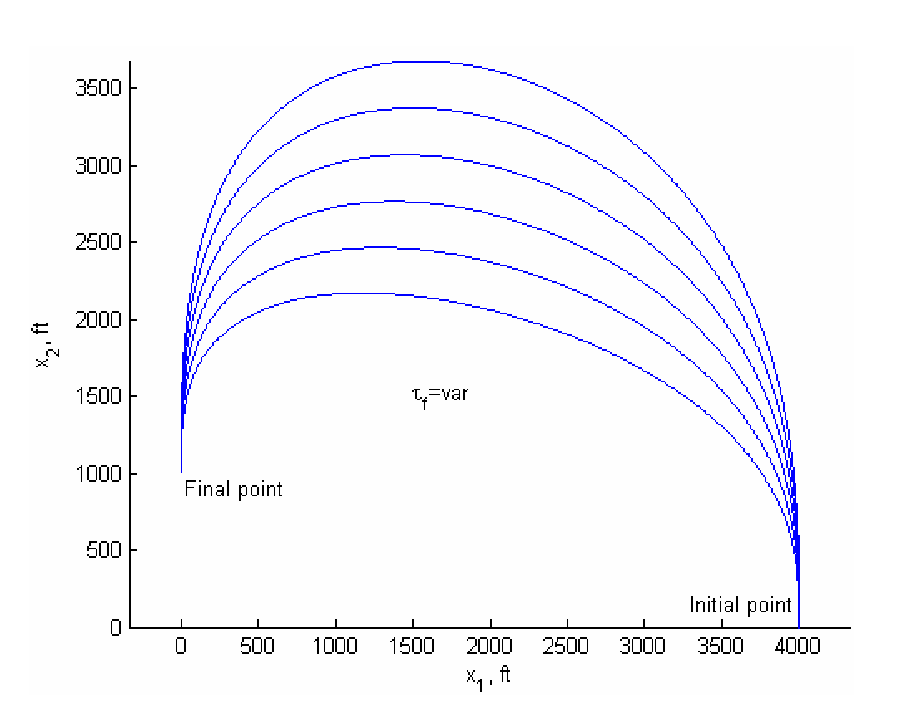
\includegraphics[width=2.5 in]{figures/poly1.eps}   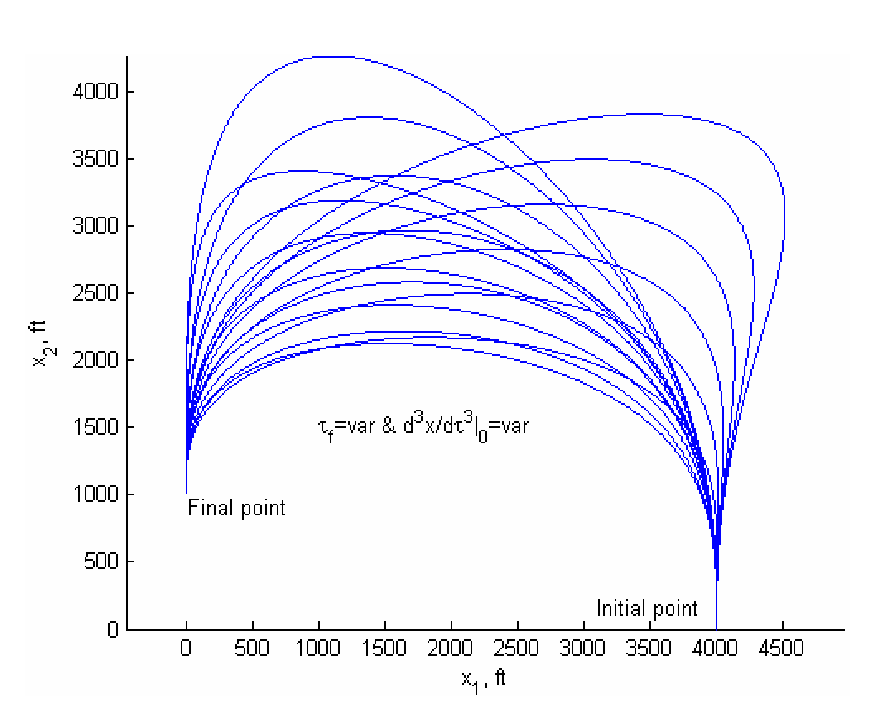
\includegraphics[width=2.5 in]{figures/poly2.eps}\\
%  \caption{Admissible trajectories for $5^{{\rm th}}$ and $6^{{\rm th}}$ order
%  polynomials.}\label{trajsim1}\end{center}
%\end{figure}
%
%\begin{figure}\begin{center}
%  % Requires \usepackage{graphicx}
%  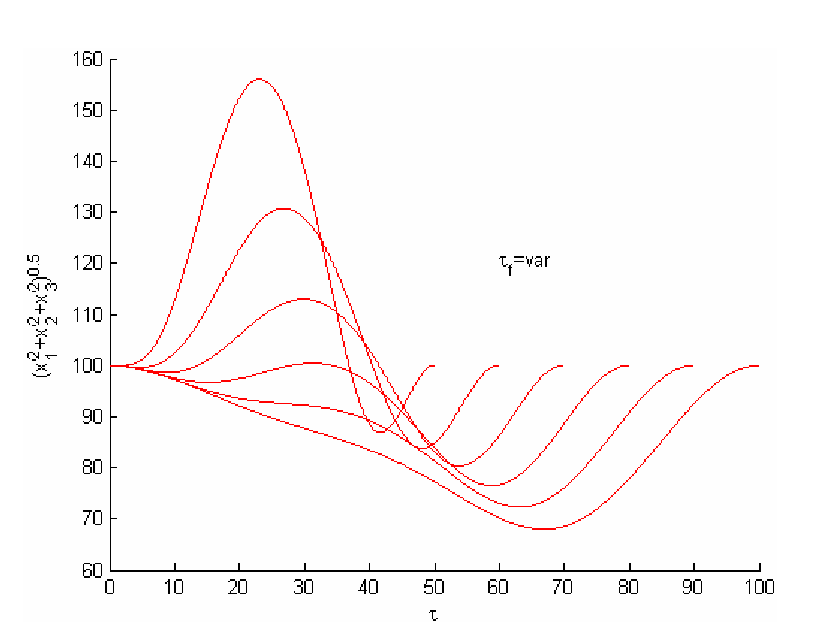
\includegraphics[width=2.6 in]{figures/traj1.eps}   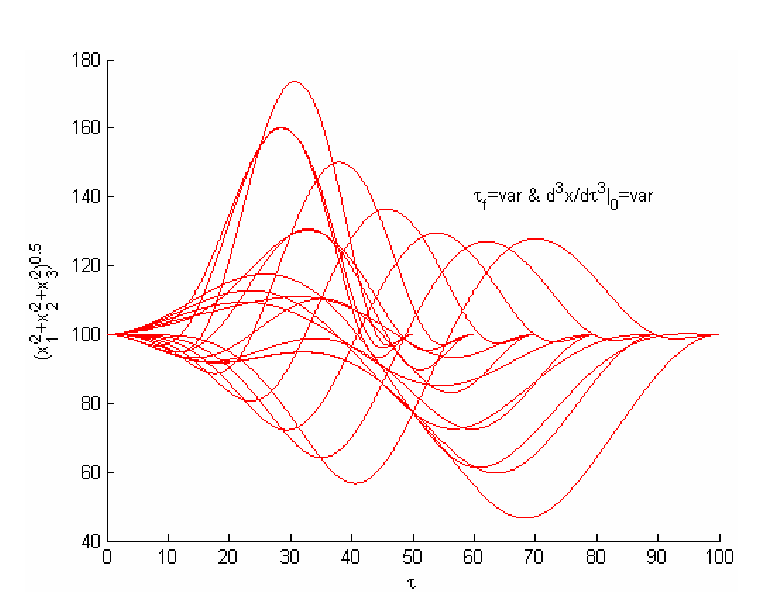
\includegraphics[width=2.6 in]{figures/traj2.eps}\\
%  \caption{Speed profile corresponding to the paths shown in Figure \ref{trajsim1} when $\tau =
%  t$. Left: varying $\tau_f$. Right: varying $\tau_f$ and the initial
%jerk.}\label{speedsims1}.
%  \end{center}
%\end{figure}

In the scope of this work we are interested in small UAVs that operate essentially at constant speeds.
Clearly, in this case speed constraints can be easily satisfied for any constant $ v_p \in [v_{{\rm min}},
v_{{\rm max}} ]$. This in turn defines

\begin{eqnarray}
\eta(\tau) &=&  \frac{v_p}{||p'_c(\tau)||} \label{defeta}\\
%\eta'(\tau)&=& -v_p \frac{(p'_c(\tau))^T p''_c(\tau)}{|| p'_c(\tau)||^3}.
\dot p_c(t) &=& v_p \frac{p'_c(\tau)}{|| p'_c(\tau)||} \label{ptau}
\end{eqnarray}

\noindent Now using (\ref{velacc}, \ref{defeta}) we obtain

\begin{eqnarray}
\ddot{p}_c(t)&=&\frac{v_p^2}{||p'_c(\tau)||^2} (I - \frac{p'_c(\tau)
(p'_c(\tau))^T}{||p'_c(\tau)||^2}) p''(\tau). \label{pptau}
\end{eqnarray}

\noindent Therefore, we can choose
\begin{eqnarray}
p'_c(0) &=& \frac{\dot p_c(0)}{||\dot p_c(0)||} \label{ptau0} \\
p'_c(\tau_f) &=& \frac{\dot p_c(t_f)}{||\dot p_c(t_f)||}.
\label{ptauf}
\end{eqnarray}
\noindent to satisfy boundary conditions on $\dot p_c(t)$. Similarly, setting
\begin{eqnarray*}
p''_c(0) &=& \ddot p_c(0) \label{pptau0} \\
p''_c(\tau_f) &=& \ddot p_c(t_f)  \label{pptauf}, \\
\end{eqnarray*}
satisfies equation (\ref{pptau}) at the boundaries.

On the other hand, the total acceleration $a_p$
of a vehicle flying along the path $p_c(\tau)$ at a constant speed is the product of the curvature of
the path with its velocity along the path squared. The curvature of the path $p_c(\tau)$ is given by
\[
\kappa(\tau) = \frac{1}{||p'(\tau)||}
||\frac{d}{d \tau} \frac {p'_c(\tau)}{||p'_c(\tau)||}||.
\]
\noindent Thus, using simple algebra it can be shown that
\begin{eqnarray*}
a_p(\tau) &=& v^2_p \kappa(\tau) \\
    &=&\frac{v_p^2}{||p'_c(\tau)||^2}
||(I - \frac{p'_c(\tau)(p'_c(\tau))^T}{||p'_c(\tau)||^2}) p''(\tau)||,
\end{eqnarray*}
\noindent which as expected is the norm of $\ddot p_c(t)$ (see equation (\ref{pptau}).
Therefore, for the case of constant
velocities $v_p$ a feasible path must satisfy the following set
of constraints

\begin{eqnarray} \label{cond1a}
v_{\rm min} \le v_p ~ \le v_{\rm max}, ~~~~ a_p(\tau) \le a_{\rm max},
~ \forall \tau \in [0,\tau_f].
\end{eqnarray}

\noindent for a pre-specified acceleration bound $a_{\rm max}$.

In this paper, we use this simple definition of a feasible path to address the problem
of a mission planning of a tactical UAV whereby the UAV must avoid detection by a radar
and accomplish the mission in a minimum time.  The approach proposed here finds a
feasible path that makes the minimum time mission planning problem easily solvable by a
single UAV flying at constant speeds along the path. Next, we make these ideas more
precise.

Let $l_{f}$ denote the total path length and $v_{p}$ denote its velocity along this
path. Then
$$
l_{f}=\int^{\tau_{f}}_0 ||p'_{c}(\tau)|| ~ d \tau.
$$
It follows immediately that the time of flight $t_{f}$ of UAV is given by
\begin{eqnarray} \nonumber t_{f_{{\rm min}}} &=&
\int^{\tau_{f}}_0 \frac{||p'_{c}(\tau)||} {v_{{\rm p}}}~ d \tau.
\end{eqnarray}
Define a cost function $J = t_{f}$. Then, making $J$ arbitrarily small over the set of
feasible paths, feasible velocities and accelerations  will result in the desired
solution to the minimal time problem discussed above. Therefore, we propose to solve
the following path generation problem

\begin{eqnarray}
F: \left\{
\begin{array}{llll}
\displaystyle{\min_{\tau_{f},v_{p}, \;} \{ J  \} } \\
subject~to
~boundary~conditions~and~limitations~(\ref{cond1a})\\
~while
\displaystyle{\min_{j = 1, \ldots, n,} ||P_{det_i}(\tau)||^2 \le E^2},
\end{array} \right.
\end{eqnarray}

Solution to the optimization problem $F$ includes an optimal paths and constant speed
profile that together minimize $J$ subject to boundary conditions and control
limitations~(\ref{cond1a}) and an additional penalty function $\Delta$ that besides
penalizing the UAV states~$\eta(\tau)$, controls~$\xi(\tau)$ and their
derivatives~$\pi(\tau)$ defines the UAV's detection probability $P_{det_i}$ by a set of
${i = 1, \ldots, n}$ radars. The choice of penalty function is what makes the
optimization task relevant to the tactical sense of the UAV mission. In application to
the task at hand it can be represented as follows:
\begin{eqnarray}\label{penalty}
\begin{array}{cr}
\Delta=\sum_{j = 1}^{k} w_j\cdot max(0;\eta-\eta_{bound})^2
         +\sum_{j = 1}^{l} w_{j+k}\cdot  max(0;\xi-\xi_{bound})^2\\\\
          +\sum_{j = 1}^{m}  w_{j+k+l}\cdot  max(0;\pi-\pi_{bound})^2
           +\sum_{i = 1}^{n}  w_{j+k+l+m+n}\cdot  max(0;P_{det_i}-P_{bound})^2
\end{array}
\end{eqnarray}
where the values of $\eta_{bound}$,$\xi_{bound}$,$\pi_{bound}$ are the design bounds
defined a priory, and $w_j$ are the weight coefficients $(\sum_{j = 1}^{j+k+l+m+n} w_j
=1)$ that are chosen heuristically to ensure specified accuracy of matching the
constraints. As a result the optimization problem is reduced to a nonlinear programming
problem with an objective of minimizing the scalar function of a limited number of
variables.

The optimization problem $F$ can be effectively solved in near real-time by
constructing a penalty function $G$ as discussed in works
\cite{Dobr1999_JCSI,JGCD00_Yakimenko} and by using any zero-order optimization
technique like the Hooke-Jeeves pattern direct-search
algorithm\cite{HookeJeevs1961_JACM} or Nelder-Mead downhill simplex
algorithm\cite{NelderMead1965_TCJ}. In the task at hand the Hooke-Jeeves optimization
algorithm was implemented online at $4Hz$ thus producing a near optimal solution not
faster than 4 times a second. Constraining the update rate of the optimization code
allowed balancing the computational load of the onboard CPU.

A particular example of tactical UAV mission solved by utilizing the path generation
algorithm will be provide later in the experimental results section.

%As an example, Fig.~\ref{ex1} illustrates the flexibility afforded by the reference
%polynomials to compute a coordinated target reconnaissance mission by three UAVs. In
%this case, the vector of optimization parameters is $\Xi = [\tau_{f1} ~~ \tau_{f2} ~~
%\tau_{f3} ~~ v_{p_1} ~~ v_{p_2}~~ v_{p_3}]$. The final value of the cost function $J =
%1.6968e-006$ corresponds to $|\max_i t_{fi} - \min_i t_{fi}| \le ~~ 0.0013 ~~ sec$. The
%value of the optimization parameter vector $\Xi_{final} = [4010.0 ~~ 4999.7 ~~ 7487.6
%~~ 15.1380 ~~ 21.2238 ~~ 29.8054]$ resulted in spatially deconflicted paths where the
%minimum distance between any two paths did not fall below $350 ~ m$ (the minimum
%required distance was $100 ~ m$). The optimal speed profiles $[15.1380~m/s ~~
%21.2238~m/s ~~ 29.8054~m/s]$ are well within predefined limits of $v_{{\rm min}},
%v_{{\rm max}}$ were $15 m/sec$ and $30 m/sec$, respectively.
%%The selected speed limits were
%%well inside the physical capabilities of the UAVs used in the flight
%%tests.
%%This was done to ensure that each path can be tracked in
%%the presence of winds.
%The maximum acceleration corresponding to
%each path did not exceed $0.89 m/sec^2$, well below the limit of
%$0.5 g$.  Finally, the resulting total path lengths for each path were
%$[ \l_{f1} ~~ \l_{f2} ~~ \l_{f3} ] = [4535.4 ~~ 6358.7  ~~ 8929.7]$.




%\begin{figure}
%  % Requires \usepackage{graphicx}
%  \begin{center}
%  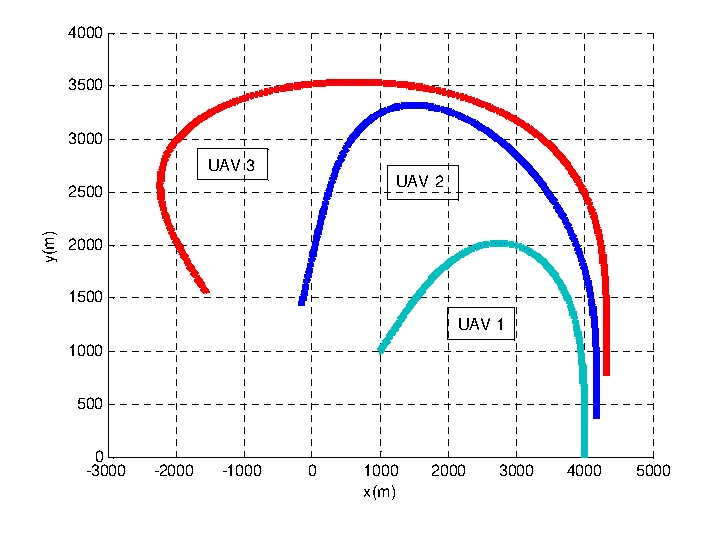
\includegraphics[width=3in]{traj3.eps}
%  \includegraphics[width=3.2in]{traj4.eps}
%  \caption{Example of spatially deconflicted trajectories. Top view, moving from right to left (left), 3D
% view, moving from left to right (right).}\label{ex1}
%\end{center} \end{figure}
%
%
%\begin{figure}
%  % Requires \usepackage{graphicx}
%  \begin{center}
%  \includegraphics[width=3.1in]{traj6.eps}\\
%  \caption{Intersection of time intervals $T_i$ for each UAV.}\label{ex3}
%\end{center} \end{figure}



\begin{thebibliography}{9}% maximum number of references (for label width)
\bibitem{JGCD00_Yakimenko}
    Yakimenko, O. A.,
    \newblock Direct method for rapid prototyping of near-optimal aircraft trajectories.
    \newblock {\em AIAA Journal of Guidance, Control, \& Dynamics}, 23(5):865--875,2000.

\bibitem{JGCD10_PFL1aug},
    Kaminer I.I., Pascoal A.M., Xargay E.M., Hovakimyan N., Cao C.C., Dobrokhodov V.N.,
    \newblock Path Following for Unmanned Aerial Vehicles using {$\mathcal{L}_1$}~Adaptive Augmentation of Commercial Autopilots",
    \newblock {\emph{AIAA Journal of Guidance, Control \& Dynamics}}, 33(2):550-564,2010

\bibitem{Dobr1999_JCSI}
    Dobrokhodov,V. N., and Yakimenko, O. A.,
    \newblock Synthesis of Trajectorial Control Algorithms at the Stage of Rendezvous of an Airplane with a ManeuveringObject,
    \newblock {\emph{Journal of Computer and Systems Sciences International}}, 38(2):262–277, 1999.

\bibitem{HookeJeevs1961_JACM}
    Hooke, R., and Jeeves, T. A.,
    \newblock ‘Direct Search’ Solution of Numerical and Statistical Problems,
    \newblock {\emph{Journal of the Association for Computing Machinery}}, 8(2):212-229,1961

\bibitem{NelderMead1965_TCJ}
    Nelder, J. A., and Mead, R.,
    \newblock A Simplex Method for Function Minimization,
    \newblock {The Computer Journal}, 8(7):308-313, 1965.
\end{thebibliography}


\end{document}

% $Id: template_basic.tex,v 1.5 2004/05/23 12:49:44 kleb Exp $
